\begin{figure}[htbp]
  \centering
  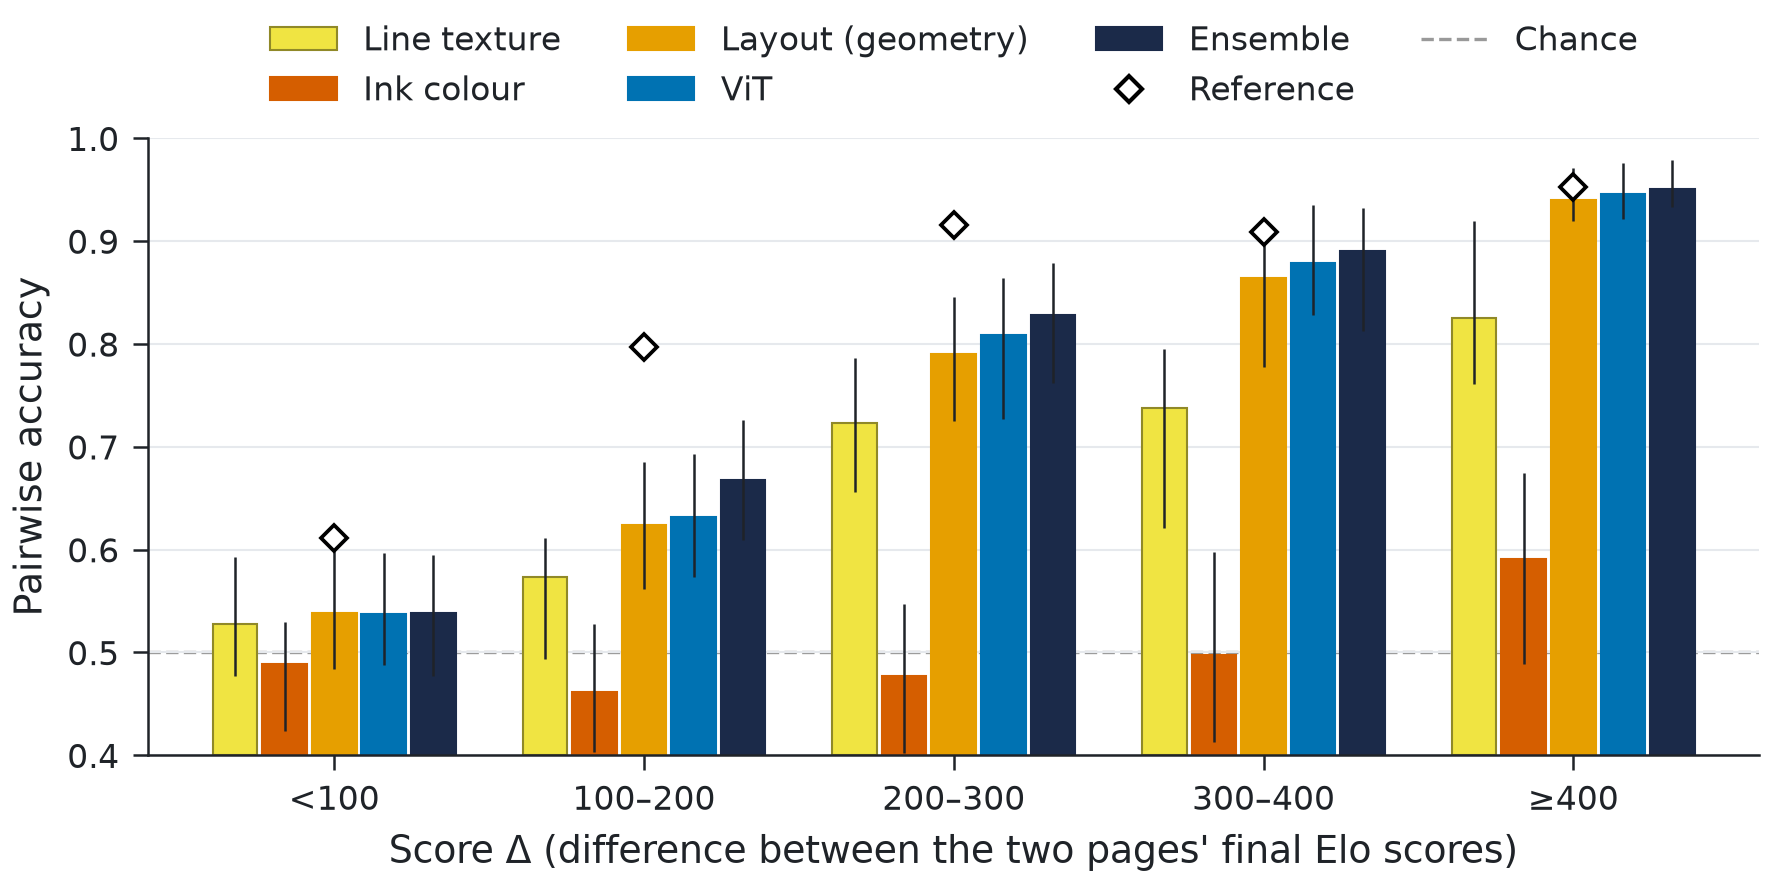
\includegraphics[width=15.00cm]{figures/accuracy_by_elo_gap.png}
  \caption{Pairwise accuracy on the test judgements by the absolute difference ($\Delta$) between the two pages' final Elo scores: \emph{Line texture}, the pairwise logistic model on the 38 line-texture features; \emph{Ink colour}, the pairwise logistic model on the seven ink colour measures, chromatic share, hue classes, hue entropy, saturation, colour by zone, colour across lines and coloured initials (17 columns); \emph{Layout (geometry)}, the pairwise logistic model on the 83 geometric features; \emph{ViT}, the local scoring head on the patch tokens of DINOv2 ViT-S/14 (block 12, 518 pixels on the long edge, the folio crop): an MLP (384--128--1, ReLU, softplus) scoring each patch, the page's score the mean of its patches', trained with RankNet's logistic loss (180 epochs of Adam); \emph{Ensemble}, the mean of the z-scored page scores of \emph{Layout (geometry)} and \emph{ViT}. Bars are the mean over the folds, whiskers 95\% intervals from 1,000 resamples of the manuscripts; diamonds the Reference, the consistency of the same test judgements with the final Elo scores (the share that agree with them), the limit for accuracy; the dashed line chance. Each method is evaluated by 10-fold cross-validation repeated 10 times, each manuscript's pages in one fold; a fold tests the judgements between two of its pages.}
  \label{fig:accuracy_by_elo_gap}
\end{figure}
